\documentclass[12pt]{article}
\usepackage{algo,fullpage,url,amssymb,epsfig,color,xspace,tikz,amsmath,rotating,qtree}
\usepackage{graphicx}
\usepackage[pdftitle={CS 240 Assignment 5},
pdfsubject={University of Waterloo, CS 240, Spring 2014},
pdfauthor={Romain Lebreton}]{hyperref}

%%%%%%%%%%%%%%%%%%%%% TIKZ %%%%%%%%%%%%%%%%%%%%%%%%%%%%%%
\usepackage{tkz-graph}
\usepackage{tikz}
\usetikzlibrary{chains}

% \snode{ID}{NUMBER} becomes \node{ID}[item]{\ensuremath{NUMBER}}
\newcommand{\snode}[2]{\node(#1)[item]{\ensuremath{#2}}}
\newcommand{\hlsnode}[2]{\node(#1)[item, fill = red!30]{\ensuremath{#2}}}

% \nodelabel{SUBSCRIPT} becomes \node[label]{\ensuremath{S_SUBSCRIPT}}
\newcommand{\nodelabel}[1]{\node[label]{\ensuremath{S_#1}}}
%%%%%%%%%%%%%%%%%%%%%%%%%%%%%%%%%%%%%%%%%%%%%%%%%%%%%%%%%

\renewcommand{\thesubsection}{Problem \arabic{subsection}}

\newcommand{\vs}{\textvisiblespace}

\begin{document}

\begin{center}
  {\Large\bf University of Waterloo}\\ \vspace{3mm}
  {\Large\bf CS240, Spring 2014}\\ \vspace{2mm}
  {\Large\bf Assignment 5 - Update 1}\\ \vspace{3mm}
  \textbf{Due Date: Wednesday, July 30, at 9:15am}
\end{center}

\definecolor{care}{rgb}{0,0,0}
\def\question#1{\item[\bf #1.]}
\def\part#1{\item[\bf #1)]}
\newcommand{\pc}[1]{\mbox{\textbf{#1}}} % pseudocode

%%%% NEW %%%
\textbf{Update 1: } We have added Problems 4 to 10 to cover
range queries (module 7), text algorithms (module 8) and
compression (module 9).
All questions are written problems except problem 4.a) which is
is a programming problem; submit your solution to 4.a) electronically
as a file named {\tt kdpartition.cpp}.
%%%%%%%%%%%%

Please read
\url{http://www.student.cs.uwaterloo.ca/~cs240/s14/guidelines.pdf} for
guidelines on submission.
Submit your solutions to written problems electronically as a PDF file with
name {\tt a05wp.pdf} using MarkUs. We will also accept individual
question files named {\tt a05q1w.pdf}, {\tt a05q2w.pdf}, $\dots$.

%%%%%%%%%%%%%%%%%%%%%%%%%%%%%%%%%%%%%%%%%%%%%%%%%%%%%%%%%%%%%%%%%%%%%%%%
\subsection{Hashing [3+3=6 marks]}
Consider a hash table dictionary with universe $U=\{0, 1, 2, \dots , 24\}$ and size $M =5$. If items with keys $k = 21, 3, 16, 1$ are inserted in that order, draw the resulting hash table if we resolve collisions using:
\begin{itemize}
\item Linear probing with $h(k) = (k+1)~mod~5$\\
\begin{tabular}{c|c|}
  \hline
  0 & 1\\
  \hline
  1 & \\
  \hline
  2 & 21\\
  \hline
  3 & 16\\
  \hline
  4 & 3\\
  \hline
\end{tabular}
\item  Cuckoo hashing with $h_1(k) = k~mod~5$ and $h_2(k) =\lfloor k/5 \rfloor$ \\
\begin{tabular}{c|c|}
  \hline
  0 & 3\\
  \hline
  1 & 1\\
  \hline
  2 & \\
  \hline
  3 & 16\\
  \hline
  4 & 21\\
  \hline
\end{tabular}
\end{itemize}

%%%%%%%%%%%%%%%%%%%%%%%%%%%%%%%%%%%%%%%%%%%%%%%%%%%%%%%%%%%%%%%%%%%%%%%%
\subsection{Skip Lists [6+6+8=20 marks]}

\begin{figure}[!h]
  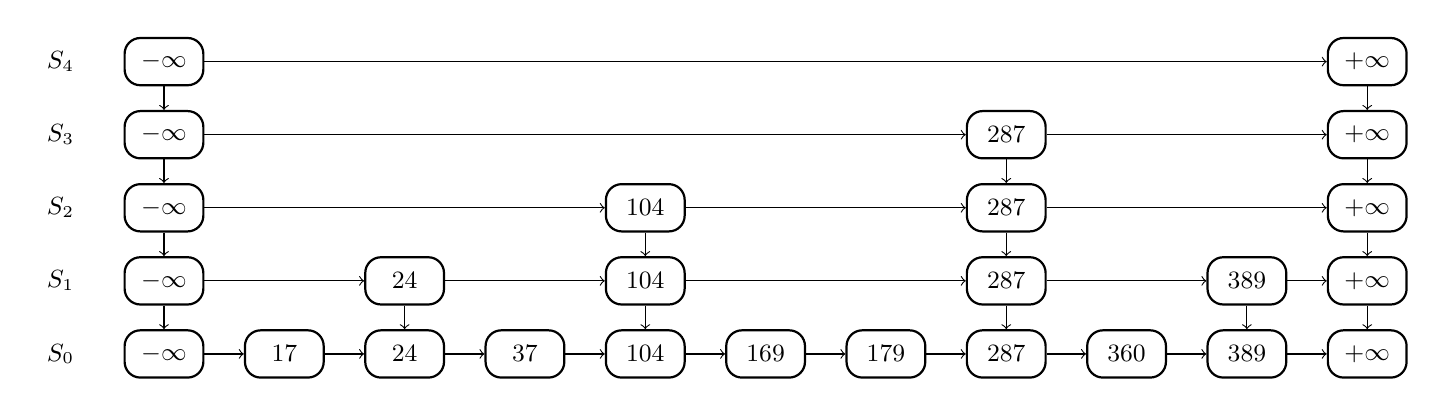
\begin{tikzpicture}[
      start chain,
      every node/.style={font=\small},
      item/.style={rectangle,minimum height=6mm,minimum width=10mm,
        rounded corners=2mm,thick,draw=black},
      label/.style={rectangle,minimum size=6mm},
      every join/.style={->}]
    % The nodes of the skip list are drawn in a matrix
    % \\ delimits the rows while & delimits the columns
    \matrix[row sep=3mm, column sep=5mm]{
      % Row 4: -infty ... +infty
      \nodelabel{4}; & \snode{4a}{-\infty}; & & & & & & & & & &\snode{4k}{+\infty};\\

      % Row 3: -infty ... 287 ... +infty
      \nodelabel{3}; & \snode{3a}{-\infty}; & & & & & & & \snode{3h}{287}; & & & \snode{3k}{+\infty};\\

      % Row 2: -infty ... 104 ... 287 ... +infty
      \nodelabel{2}; & \snode{2a}{-\infty}; & & & & \snode{2e}{104}; & & & \snode{2h}{287}; & & & \snode{2k}{+\infty};\\

      % Row 1: -infty - 24 - 104 - - 287 - 389 +infty
      \nodelabel{1}; & \snode{1a}{-\infty}; & & \snode{1c}{24}; & & \snode{1e}{104}; & & & \snode{1h}{287}; & & \snode{1j}{389}; & \snode{1k}{+\infty};\\

      % Row 0: -infty 17 24 37 104 169 179 287 360 389 +infty
      \nodelabel{0}; & \snode{0a}{-\infty}; & \snode{0b}{17}; & \snode{0c}{24}; & \snode{0d}{37}; & \snode{0e}{104}; & \snode{0f}{169}; & \snode{0g}{179}; & \snode{0h}{287}; & \snode{0i}{360}; & \snode{0j}{389}; & \snode{0k}{+\infty};\\
    };

    % Start chaining the nodes together
    {
      % Horizontal chains
      % Specify a starting node (by ID), and join to other nodes (by going "through" them in an unbroken line)
      % Eg row 2: Start at 2a, join 2e, join 2h, join 2i
      [start chain] \chainin(0a); \chainin(0b) [join]; \chainin(0c) [join]; \chainin(0d) [join]; \chainin(0e) [join]; \chainin(0f) [join]; \chainin(0g) [join]; \chainin(0h) [join]; \chainin(0i) [join]; \chainin(0j) [join]; \chainin(0k) [join];
      [start chain] \chainin(1a); \chainin(1c) [join]; \chainin(1e) [join]; \chainin(1h) [join]; \chainin(1j) [join]; \chainin(1k) [join];
      [start chain] \chainin(2a); \chainin(2e) [join]; \chainin(2h) [join]; \chainin(2k) [join];
      [start chain] \chainin(3a); \chainin(3h) [join]; \chainin(3k) [join];
      [start chain] \chainin(4a); \chainin(4k) [join];
    }
    {
      % Vertical chains
      % Need to be separate chains from the horizontal ones
      [start chain] \chainin(4a); \chainin(3a) [join]; \chainin(2a) [join]; \chainin(1a) [join]; \chainin(0a) [join];
      [start chain] \chainin(1c); \chainin(0c) [join];
      [start chain] \chainin(2e); \chainin(1e) [join]; \chainin(0e) [join];
      [start chain] \chainin(3h); \chainin(2h) [join]; \chainin(1h) [join]; \chainin(0h) [join];
      [start chain] \chainin(1j); \chainin(0j) [join];
      [start chain] \chainin(4k); \chainin(3k) [join]; \chainin(2k) [join]; \chainin(1k) [join]; \chainin(0k) [join];
    }
  \end{tikzpicture}
\end{figure}

\begin{enumerate}
\part{a} Consider the skip-list $S$ shown above. Show how $Search(S, 360)$
and  $Search(S, 17)$ proceeds.
More specifically show at which order search visits the nodes of the skip list.
Give only the successful search path, that is only the nodes that result into a 'go right' or 'go down'.
You should refer to the nodes using their keys and levels, e.g.,
you can say node 104 at level 1. The lowest level is $0$.\\
Search(S, 360)
\begin{enumerate}
  \item node -$\infty$ at level $S_4$
  \item node -$\infty$ at level $S_3$
  \item node 287 at level $S_3$
  \item node 287 at level $S_2$
  \item node 287 at level $S_1$
  \item node 287 at level $S_0$
  \item node 360 at level $S_0$
\end{enumerate}
Search(S, 360)
\begin{enumerate}
  \item node -$\infty$ at level $S_4$
  \item node -$\infty$ at level $S_3$
  \item node -$\infty$ at level $S_2$
  \item node -$\infty$ at level $S_1$
  \item node -$\infty$ at level $S_0$
  \item node 17 at level $S_0$
\end{enumerate}

\part{b} Starting with an empty skip list, insert the seven keys
      $54, 15, 51,53, 47,68,36$.
      Draw your final answer as on the figure in 4(a).
      Use the following coin
      tosses to determine the  heights of towers (note, not every
      toss is necessarily used):
     $$T,T,H,H,T,H,T,H,H,T,H,H,T,T,H,T,H,H,T,T,H,H,H,T,\ldots$$

 \begin{figure}[h]
  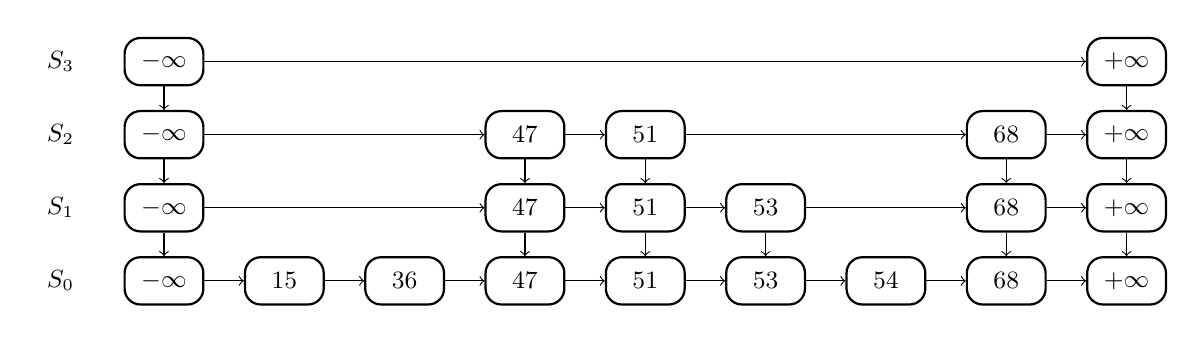
\begin{tikzpicture}[
      start chain,
      every node/.style={font=\small},
      item/.style={rectangle,minimum height=6mm,minimum width=10mm,
        rounded corners=2mm,thick,draw=black},
      label/.style={rectangle,minimum size=6mm},
      every join/.style={->}]
    \matrix[row sep=3mm, column sep=5mm]{
      \nodelabel{3}; & \snode{3a}{-\infty}; &  &  &  &  &  &  &  & \snode{3i}{+\infty};\\
      \nodelabel{2}; & \snode{2a}{-\infty}; &  &  & \snode{2d}{47}; & \snode{2e}{51}; &  &  & \snode{2h}{68}; & \snode{2i}{+\infty};\\
      \nodelabel{1}; & \snode{1a}{-\infty}; &  & & \snode{1d}{47}; & \snode{1e}{51}; & \snode{1f}{53}; &  & \snode{1h}{68}; & \snode{1i}{+\infty};\\
      \nodelabel{0}; & \snode{0a}{-\infty}; & \snode{0b}{15}; & \snode{0c}{36}; & \snode{0d}{47}; & \snode{0e}{51}; & \snode{0f}{53}; & \snode{0g}{54}; & \snode{0h}{68}; & \snode{0i}{+\infty};\\
    };

    {
      [start chain] \chainin(0a); \chainin(0b) [join]; \chainin(0c) [join]; \chainin(0d) [join]; \chainin(0e) [join]; \chainin(0f) [join]; \chainin(0g) [join]; \chainin(0h) [join]; \chainin(0i) [join];
      [start chain] \chainin(1a); \chainin(1d) [join]; \chainin(1e) [join]; \chainin(1f) [join]; \chainin(1h) [join]; \chainin(1i) [join];
      [start chain] \chainin(2a); \chainin(2d) [join]; \chainin(2e) [join]; \chainin(2h) [join]; \chainin(2i) [join];
      [start chain] \chainin(3a); \chainin(3i) [join];
    }
    {
      % Vertical chains
      % Need to be separate chains from the horizontal ones
      [start chain] \chainin(3a); \chainin(2a) [join]; \chainin(1a) [join]; \chainin(0a) [join];
      [start chain] \chainin(2d); \chainin(1d) [join]; \chainin(0d) [join];
      [start chain] \chainin(2e); \chainin(1e) [join]; \chainin(0e) [join];
      [start chain] \chainin(1f); \chainin(0f) [join];
      [start chain] \chainin(2h); \chainin(1h) [join]; \chainin(0h) [join];
      [start chain] \chainin(3i); \chainin(2i) [join]; \chainin(1i) [join]; \chainin(0i) [join];
    }
  \end{tikzpicture}
\end{figure}

\part{c} The worst case time for searching in a singly linked list
      is $\Theta(n)$.   Now consider a variation of  a skip list which
      has fixed height $h=3$ even though $n$ can become arbitrarily large.
      Level $S_0$ contains the keys $-\infty,k_1,k_2,\ldots,k_n,\infty$.
      Level $S_3$ contains only $-\infty$ and $\infty$.
      Describe subsets of keys that should be included in levels $S_1$
      and $S_2$ so that searching in the skip list has worst case cost
      $\Theta(n^{1/3})$.

      The $S_2$ layer contains multiples of $n^{\frac{2}{3}}$ this means that you will have to move left at most $\frac{n}{n^{\frac{1}{3}}} = n^{\frac{1}{3}}$ values. Then the $s_3$ layer contains multiples of $n^{\frac{1}{3}}$ this means that you will have to move left at most $\frac{n^{\frac{2}{3}}}{n^{\frac{1}{3}}} = n^{\frac{1}{3}}$ times.
      Finally you have to go through $n^{\frac{1}{3}}$ elements on the bottom row (else you would have moved over in the previous level). This means each search will go through at most $3n^{\frac{1}{3}}$ nodes before it gets to the desired spot. This has a worst case time complexity of $\Theta(n^{\frac{1}{3}})$
\end{enumerate}

%%%%%%%%%%%%%%%%%%%%%%%%%%%%%%%%%%%%%%%%%%%%%%%%%%%%%%%%%%%%%%%%%%%%%%%%
\subsection{Quad Trees [5+5=10 marks]}
For both parts of this question, use the convention that each
internal node of a quad tree has exactly four children, corresponding
to regions $NW$, $NE$, $SW$ and $SE$, in that order.

\begin{enumerate}
\part{a} One of the applications of quad trees is for image
compression.  An image (picture) is recursively divided into quadrants
until the entire quadrant is only one color.  Using this rule,
draw the quad tree of the following image.  There are only three
colors (shades of gray).  For the leaves of the quad tree, use 1
to denote the lightest shade, 2 for the middle shade and 3 for the
darkest shade of gray.
\begin{center}
  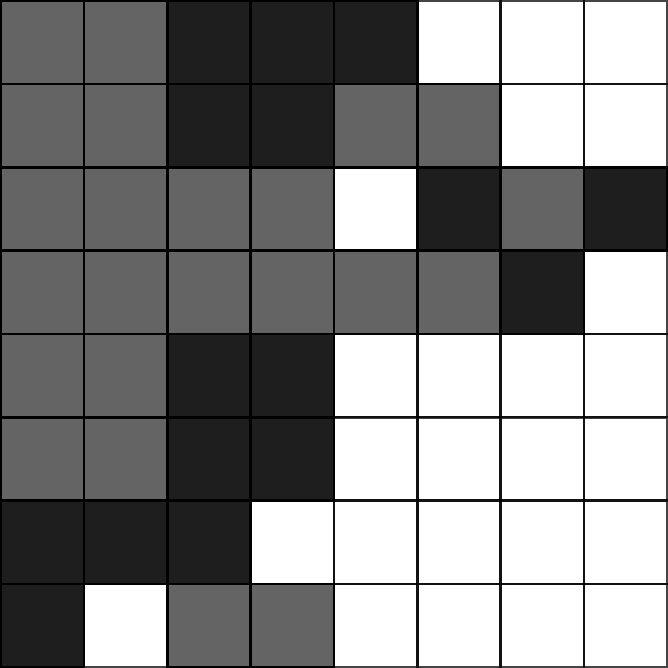
\includegraphics[width=3in]{QuadTreePic}
\end{center}
\begin{center}
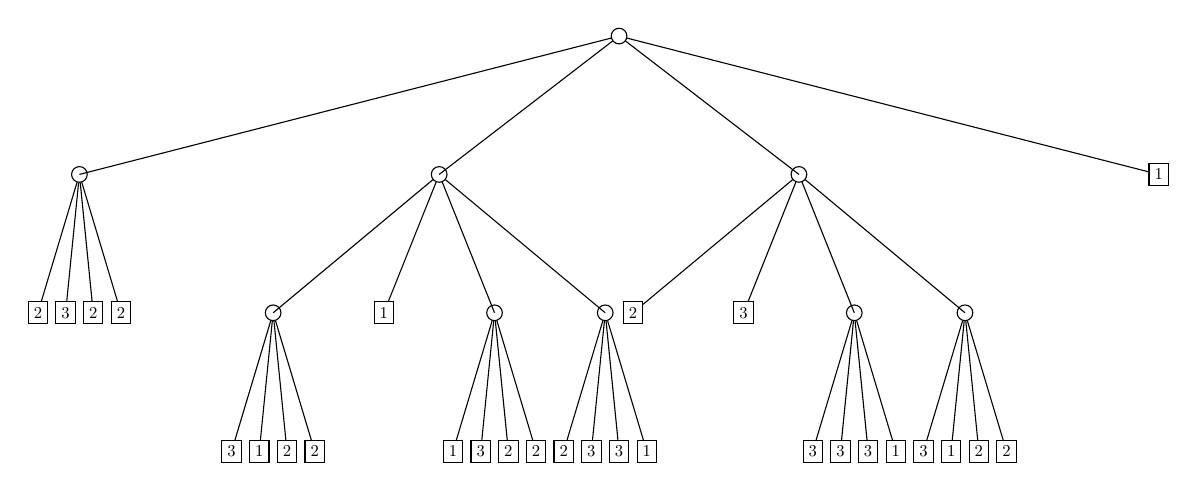
\begin{tikzpicture}[level distance=50pt,
      every node/.style={,circle,draw,scale=0.6},
      level 1/.style={sibling distance=130pt}]%,
      % level 2/.style={sibling distance=40pt},
      % level 3/.style={sibling distance=10pt}]
      \node{}
      child{ [sibling distance=10pt]
        node{}
        child{
          node[rectangle]{2}
        }
        child{
          node[rectangle]{3}
        }
        child{
          node[rectangle]{2}
        }
        child{
          node[rectangle]{2}
        }
      }
      child{ [sibling distance=40pt]
        node{}
        child{ [sibling distance=10pt]
          node{}
          child{
            node[rectangle]{3}
          }
          child{
            node[rectangle]{1}
          }
          child{
            node[rectangle]{2}
          }
          child{
            node[rectangle]{2}
          }
        }
        child{
          node[rectangle]{1}
        }
        child{ [sibling distance=10pt]
          node{}
          child{
            node[rectangle]{1}
          }
          child{
            node[rectangle]{3}
          }
          child{
            node[rectangle]{2}
          }
          child{
            node[rectangle]{2}
          }
        }
        child{ [sibling distance=10pt]
          node{}
          child{
            node[rectangle]{2}
          }
          child{
            node[rectangle]{3}
          }
          child{
            node[rectangle]{3}
          }
          child{
            node[rectangle]{1}
          }
        }
      }
      child{ [sibling distance=40pt]
        node{}
        child{
          node[rectangle]{2}
        }
        child{
          node[rectangle]{3}
        }
        child{ [sibling distance=10pt]
          node{}
          child{
            node[rectangle]{3}
          }
          child{
            node[rectangle]{3}
          }
          child{
            node[rectangle]{3}
          }
          child{
            node[rectangle]{1}
          }
        }
        child{ [sibling distance=10pt]
          node{}
          child{
            node[rectangle]{3}
          }
          child{
            node[rectangle]{1}
          }
          child{
            node[rectangle]{2}
          }
          child{
            node[rectangle]{2}
          }
        }
      }
      child{
        node[rectangle]{1}
      }
      ;
\end{tikzpicture}
\end{center}
\part{b} Give three 2-dimensional points such that the corresponding
quad tree has height exactly 9.  Give the (x,y) coordinates of the
three points and show the quad tree.  (Do not give the plane
partition.)

(0,512), (1,512), (512,512).

\begin{tikzpicture}[level distance=30pt,
      every node/.style={,circle,draw,scale=0.6},
      ]
      \node{}
      child {
        node{512,512}
      }
      child{
        node{}
        child{
        edge from parent[draw=none]
        }
        child {
          node{}
          child{
            edge from parent[draw=none]
          }
          child {
            node{}
              child{
                edge from parent[draw=none]
              }
              child {
                node{}
                child{
                  edge from parent[draw=none]
                }
                child {
                  node{}
                  child{
                    edge from parent[draw=none]
                  }
                  child {
                    node{}
                      child{
                        edge from parent[draw=none]
                      }
                      child {
                        node{}
                        child{
                          edge from parent[draw=none]
                        }
                        child {
                          node{}
                          child{
                            node{0,512}
                          }
                          child {
                            node{1,512}
                          }
                          edge from parent node[right, draw=none]
                        }
                        edge from parent node[right, draw=none]
                      }
                    edge from parent node[right, draw=none]
                  }
                  edge from parent node[right, draw=none]
                }
                edge from parent node[right, draw=none]
              }
            edge from parent node[right, draw=none]
          }
          edge from parent node[right, draw=none]
        }
      };
\end{tikzpicture}


\end{enumerate}

%%%%%%%%%%%%%%%%%%%%%%%%%%%%%%%%%%%%%%%%%%%%%%%%%%%%%%%%%%%%%%%%%%%%%%%%
\subsection{$kd$-Tree Construction [15+5=20 marks]}
\begin{enumerate}
\part{a} Implement an $O(n\log n)$ algorithm to construct a $kd$-tree
for dimension 2.  Your algorithm should read $2n+1$ integers from
standard input, separated by white space or carriage return.  The first integer is the
number of points.  The remaining $2n$ integers are the $n$ points
themselves, according to their $x$ and $y$ coordinates.

Use the recipe on Slide 13 of Module 7 with the following modification on the split:
If the array $Px[0..n-1]$ for $n>1$ is storing points
sorted in increasing order according to their $x$-coordinate, then
the vertical splitting line goes through point $Px[mid]$, where
$mid = \lfloor n/2\rfloor$.  The root node contains $Px[mid]$, the
region to the left of the splitting
line include the points $Px[0..mid-1]$, and the region the the
right of the splitting line includes the points $Px[mid+1..n-1]$.

As explained in class, the idea of the algorithm is to first do some
preprocessing: sort the points on both their $x$ and $y$ coordinates.
For this preprocessing step you may use a standard library function;
assume that the sorting algorithm runs in time $O(n\log n)$. You may
also need some additional preprocessing.  Then call a recursive function
(which you create) to produce a tree like the one of Slide 14 of Module 7.
Actually, your program does not need to construct the tree, but rather
should just print to standard output the $n$ points stored in the nodes
of the tree in the order they are visited during an in-order traversal.
The coordinates of the point must be separated by a white space and we want
one point per line.

Here is an example input:
\begin{verbatim}
3
3 4
2 2
1 1
\end{verbatim}
The points are $p_0,p_1,p_2 = (3,4),(2,2),(1,1)$. These three
points correspond to the following $kd$-tree:

\hfill
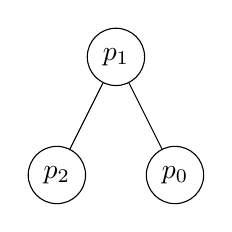
\begin{tikzpicture}[every node/.style={circle,draw}]
\node{$p_1$}
 child{ node{$p_2$}}
 child{ node{$p_0$}}
 ;
\end{tikzpicture}
\hfill \resizebox{30mm}{!}{\input{kdtreeExample.pdf_tex}}
\hfill \phantom{a}

Thus, for this example your algorithm should print out:
\begin{verbatim}
1 1
2 2
3 4
\end{verbatim}
Your program {\bf must} run in time $O(n \log n)$.

To avoid all ambiguity in the construction of the k-d tree, you can assume that
there will only be one point on each separating line.
Therefore the choice of the median will always be unique,
unlike the example of Slide 14 of Module 7 where $p_5$ and $p_6$ are on the same separating line.
We will test your program only on such inputs.

\part{b} Justify the $O(n \log n)$ running time of your algorithm.

One way to do this is to show that, after a preprocessing that involves sorting,
you have a recursive algorithm whose running time on a sub-problem with $k$ points
satisfies the following recurrence:
$$T(k) \leq T(\lfloor k/2\rfloor) + T(\lceil k/2 \rceil-1)+ O(k).$$
In other words, if you are splitting the region with a
vertical line according to $x$-coordinate,
explain how you produce the two sets of points in each
region sorted according to their $y$-coordinate in time $O(k)$.

Everytime through the algorithm it sorts all points using a STL algorithm sort (I assume it uses a variation of quick sort and thus has a time complexity of $O(k\log k)$) then it calls the algorithm twice on half of the array and half of the array minus one, but this time operating in the y axis. This results in the above recurrence occurance (estimating the time complexity of sorting to $O(k)$). This time recurrence will boil down to $O(n\log n)$.
\end{enumerate}

%%%%%%%%%%%%%%%%%%%%%%%%%%%%%%%%%%%%%%%%%%%%%%%%%%%%%%%%%%%%%%%%%%%%%%%%
\subsection{Range tree [5+5+5=15 marks]}
\begin{enumerate}
\part{a} Draw the unique 2-dimensional range tree corresponding to points
$[ 3, 4 ]$, $[ 10, 2 ]$, $[ 9, 9 ]$, $[ 5, 7 ]$, $[ 6, 1 ]$, $[ 0, 3 ]$, $[ 1, 8 ]$.
More specifically, we want you to draw all the trees $\tau$ and $\tau_{assoc}(p)$
for every point $p$.
\begin{center}
  \includegraphics[width=12cm]{Question5a.jpg}
\end{center}
\part{b} Assume that we have a set of $n$ numbers (not necessarily integers) and we are interested only in the number of points that lie in a range rather than in reporting all of them.  Describe how a 1-dimensional range tree (i.e., a balanced binary search tree) can be modified such that a range counting query can be performed in $O(\log{n})$ time
(independent of $k$).

Have each node of the tree maintain the number of nodes a the subtree with that root has (so the number of children + 1 for the root). So when you insert into the tree you walk up to the root from the inserted node increasing the value associated with each parent. Now range search only needs to iterate down through the tree twice checking and counting each boundary node, then adding the value associated with the parent node of each internal tree. This results in a time complexity of $O(2\log n + c) \in O(\log n)$ because you iterate through the height of the tree twice (for each boundary) and preform an addition for each direct internal child.

\part{c} Now consider the 2-dimensional-case: We have a set of $n$ 2-dimensional points.  Given a query rectangle $R$, we want to find the number of points that lie in $R$.  Preprocess the $n$ points (by building an appropriate data structure) such that you can answer any of these counting queries in time $O((\log n)^2)$.

We can use the same preprocessing method as in b, but applied to each associated tree as well. The range search for the x range is still $O(\log n)$ and now for each of the $(2\log n)$ boundary check if both of the x and y values are in the range. Then run the augmented range search from b on each of the associated trees of the top inside nodes of, which there $O(\log n)$, which will also be time complexity of $O(\log n)$. The cumulative time complexity is now $O(2\log^2 n) \in O(\log^2 n)$.

\end{enumerate}

%%%%%%%%%%%%%%%%%%%%%%%%%%%%%%%%%%%%%%%%%%%%%%%%%%%%%%%%%%%%%%%%%%%%%%%%
\subsection{Tries [3+3+3+3+3=15 marks]}
\begin{itemize}
\part{a} Construct a trie on the following eight strings (include edge labels for clarity):\\ 000000, 1111111, 1111100, 011, 11011, 001111, 001100, 000100.
\begin{center}
  \begin{tikzpicture}[level distance=30pt,
      every node/.style={,circle,draw,scale=.5},
      level 1/.style={sibling distance=200pt},
      level 2/.style={sibling distance=100pt},
      level 3/.style={sibling distance=50pt},
      level 4/.style={sibling distance=25pt}]
      \node{}
      child{
        node{}
        child{
          node{}
          child{
            node{}
            child{
              node{}
              child{
                node{}
                child{
                  node{000000}
                  edge from parent node [left, draw=none]{0}
                }
                child{
                  edge from parent[draw=none]
                }
                edge from parent node [left, draw=none]{0}
              }
              child{
                  edge from parent[draw=none]
                }
              edge from parent node [left, draw=none]{0}
            }
            child{
              node{}
              child{
                node{}
                child{
                  node{000100}
                  edge from parent node [left, draw=none]{0}
                }
                child{
                  edge from parent[draw=none]
                }
                edge from parent node [left, draw=none]{0}
              }
              child{
                edge from parent[draw=none]
              }
              edge from parent node [right, draw=none]{1}
            }
            edge from parent node [left, draw=none]{0}
          }
          child{
            node{}
            child{
              edge from parent [draw=none]
            }
            child{
              node{}
              child{
                node{}
                child{
                  node{001100}
                  edge from parent node[left, draw=none]{0}
                }
                child{
                  edge from parent [draw=none]
                }
                edge from parent node[left, draw=none]{0}
              }
              child{
                node{}
                child{
                  edge from parent [draw=none]
                }
                child{
                  node{001111}
                  edge from parent node[right,draw=none]{1}
                }
                edge from parent node[right, draw=none]{1}
              }
              edge from parent node[right, draw=none]{1}
            }
            edge from parent node [right,draw=none]{1}
          }
          edge from parent node [left,draw=none]{0}
        }
        child{
          node{}
          child{
            edge from parent [draw=none]
          }
          child{
            node{011}
            edge from parent node [right, draw=none]{1}
          }
          edge from parent node [right, draw=none]{1}
        }
        edge from parent node [left, draw=none]{0}
      }
      child{
        node{}
        child{
          edge from parent [draw=none]
        }
        child{
          node{}
            child{
              node{}
              child{
                edge from parent [draw=none]
              }
              child{
                node{}
                child{
                  edge from parent [draw=none]
                }
                child{
                  node{11011}
                  edge from parent node[right, draw=none]{1}
                }
                edge from parent node[right, draw=none]{1}
              }
              edge from parent node[left, draw=none]{0}
            }
            child{
              node{}
              child{
                edge from parent [draw=none]
              }
              child{
                node{}
                child{
                  edge from parent [draw=none]
                }
                child{
                  node{}
                  child{
                    node{}
                    child{
                      node{1111100}
                      edge from parent node[left, draw=none]{0}
                    }
                    child{
                      edge from parent[draw=none]
                    }
                    edge from parent node[left, draw=none]{0}
                  }
                  child{
                    node{}
                    child{
                      edge from parent [draw=none]
                    }
                    child{
                      node{1111111}
                      edge from parent node[right, draw=none]{1}
                    }
                    edge from parent node[right, draw=none]{1}
                  }
                  edge from parent node[right, draw=none]{1}
                }
                edge from parent node[right, draw=none]{1}
              }
              edge from parent node[right, draw=none]{1}
            }
          edge from parent node[right, draw=none]{1}
        }
        edge from parent node [right, draw=none]{1}
      };
  \end{tikzpicture}
\end{center}
\part{b} Draw the compressed trie equivalent to the trie in the previous part.
\begin{center}
  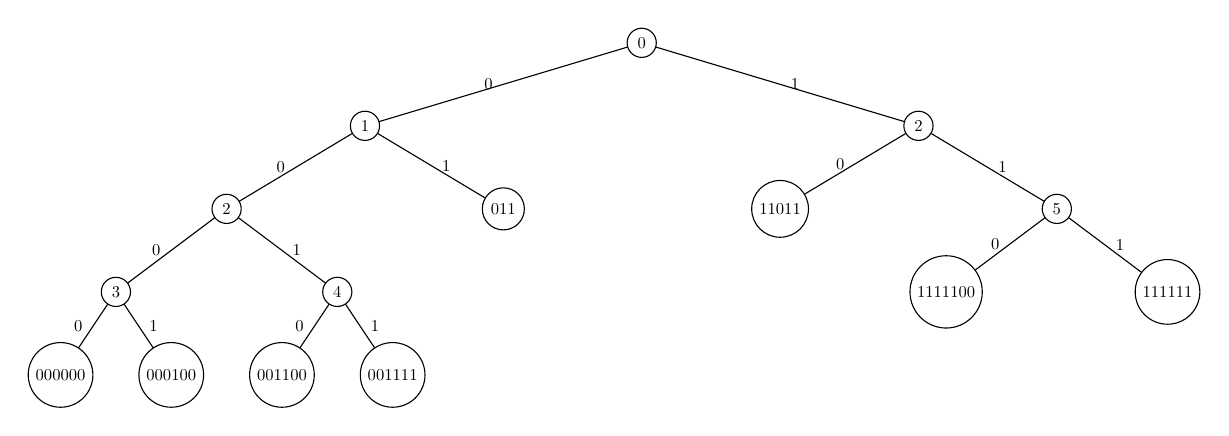
\begin{tikzpicture}[level distance=30pt,
      every node/.style={,circle,draw,scale=.6},
      level 1/.style={sibling distance=200pt},
      level 2/.style={sibling distance=100pt},
      level 3/.style={sibling distance=80pt},
      level 4/.style={sibling distance=40pt}]
      \node{0}
      child{
        node{1}
        child{
          node{2}
          child{
            node{3}
            child{
              node{000000}
              edge from parent node[left, draw=none]{0}
            }
            child{
              node{000100}
              edge from parent node[right, draw=none]{1}
            }
            edge from parent node[left, draw=none]{0}
          }
          child{
            node{4}
            child{
              node{001100}
              edge from parent node[left, draw=none]{0}
            }
            child{
              node{001111}
              edge from parent node[right, draw=none]{1}
            }
            edge from parent node[right, draw=none]{1}
          }
          edge from parent node[left, draw=none]{0}
        }
        child{
          node{011}
          edge from parent node[right, draw=none]{1}
        }
        edge from parent node[left, draw=none]{0}
      }
      child{
        node{2}
        child{
          node{11011}
          edge from parent node[left, draw=none]{0}
        }
        child{
          node{5}
          child{
            node{1111100}
            edge from parent node[left, draw=none]{0}
          }
          child{
            node{111111}
            edge from parent node[right, draw=none]{1}
          }
          edge from parent node[right, draw=none]{1}
        }
        edge from parent node[right, draw=none]{1}
      };
  \end{tikzpicture}
\end{center}
\part{c} Draw the compressed trie of the previous part after inserting 00011.
\begin{center}
  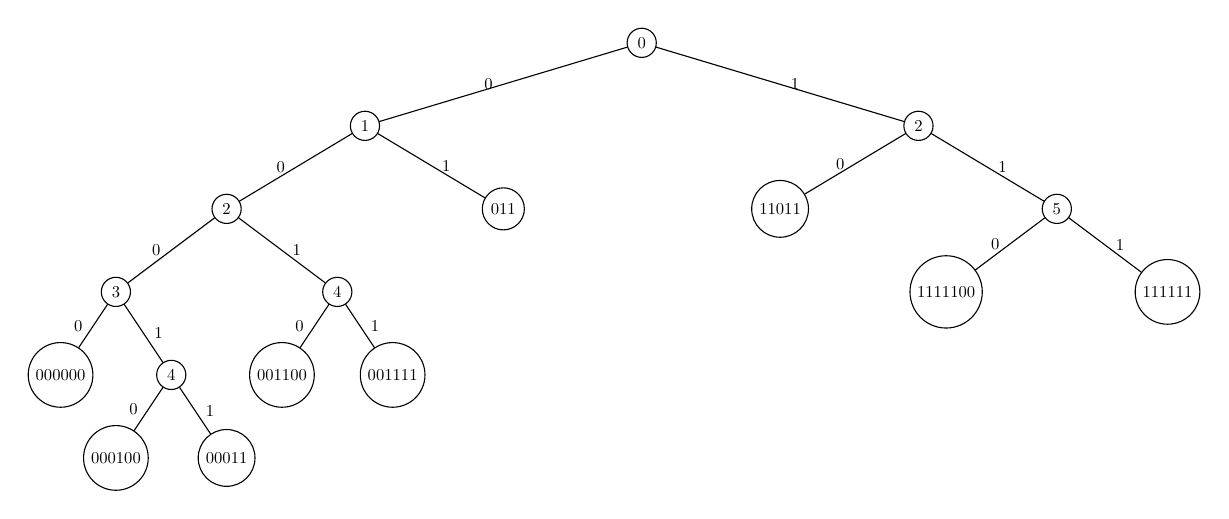
\begin{tikzpicture}[level distance=30pt,
      every node/.style={,circle,draw,scale=.6},
      level 1/.style={sibling distance=200pt},
      level 2/.style={sibling distance=100pt},
      level 3/.style={sibling distance=80pt},
      level 4/.style={sibling distance=40pt}]
      \node{0}
      child{
        node{1}
        child{
          node{2}
          child{
            node{3}
            child{
              node{000000}
              edge from parent node[left, draw=none]{0}
            }
            child{
              node{4}
              child{
                node{000100}
                edge from parent node[left, draw=none]{0}
              }
              child{
                node{00011}
                edge from parent node[right, draw=none]{1}
              }
              edge from parent node[right, draw=none]{1}
            }
            edge from parent node[left, draw=none]{0}
          }
          child{
            node{4}
            child{
              node{001100}
              edge from parent node[left, draw=none]{0}
            }
            child{
              node{001111}
              edge from parent node[right, draw=none]{1}
            }
            edge from parent node[right, draw=none]{1}
          }
          edge from parent node[left, draw=none]{0}
        }
        child{
          node{011}
          edge from parent node[right, draw=none]{1}
        }
        edge from parent node[left, draw=none]{0}
      }
      child{
        node{2}
        child{
          node{11011}
          edge from parent node[left, draw=none]{0}
        }
        child{
          node{5}
          child{
            node{1111100}
            edge from parent node[left, draw=none]{0}
          }
          child{
            node{111111}
            edge from parent node[right, draw=none]{1}
          }
          edge from parent node[right, draw=none]{1}
        }
        edge from parent node[right, draw=none]{1}
      };
  \end{tikzpicture}
\end{center}
\part{d} Draw the compressed trie of part (b) after inserting 111011.
\begin{center}
  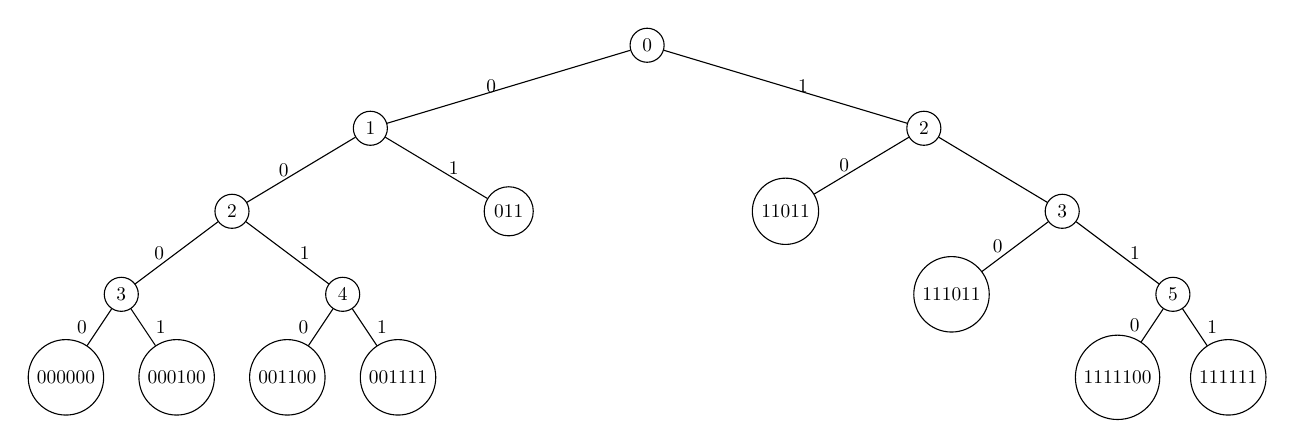
\begin{tikzpicture}[level distance=30pt,
      every node/.style={,circle,draw,scale=.7},
      level 1/.style={sibling distance=200pt},
      level 2/.style={sibling distance=100pt},
      level 3/.style={sibling distance=80pt},
      level 4/.style={sibling distance=40pt}]
      \node{0}
      child{
        node{1}
        child{
          node{2}
          child{
            node{3}
            child{
              node{000000}
              edge from parent node[left, draw=none]{0}
            }
            child{
              node{000100}
              edge from parent node[right, draw=none]{1}
            }
            edge from parent node[left, draw=none]{0}
          }
          child{
            node{4}
            child{
              node{001100}
              edge from parent node[left, draw=none]{0}
            }
            child{
              node{001111}
              edge from parent node[right, draw=none]{1}
            }
            edge from parent node[right, draw=none]{1}
          }
          edge from parent node[left, draw=none]{0}
        }
        child{
          node{011}
          edge from parent node[right, draw=none]{1}
        }
        edge from parent node[left, draw=none]{0}
      }
      child{
        node{2}
        child{
          node{11011}
          edge from parent node[left, draw=none]{0}
        }
        child{
          node{3}
          child{
            node{111011}
            edge from parent node[left, draw=none]{0}
          }
          child{
            node{5}
            child{
              node{1111100}
              edge from parent node[left, draw=none]{0}
            }
            child{
              node{111111}
              edge from parent node[right, draw=none]{1}
            }
            edge from parent node[right, draw=none]{1}
          }
        }
        edge from parent node[right, draw=none]{1}
      };
  \end{tikzpicture}
\end{center}
\part{e} Draw the compressed trie of part (b) after deleting 001100.
\begin{center}
  \begin{tikzpicture}[level distance=30pt,
      every node/.style={,circle,draw,scale=.6},
      level 1/.style={sibling distance=200pt},
      level 2/.style={sibling distance=100pt},
      level 3/.style={sibling distance=80pt},
      level 4/.style={sibling distance=40pt}]
      \node{0}
      child{
        node{1}
        child{
          node{2}
          child{
            node{3}
            child{
              node{000000}
              edge from parent node[left, draw=none]{0}
            }
            child{
              node{000100}
              edge from parent node[right, draw=none]{1}
            }
            edge from parent node[left, draw=none]{0}
          }
          child{
            node{001111}
            edge from parent node[right, draw=none]{1}
          }
          edge from parent node[left, draw=none]{0}
        }
        child{
          node{011}
          edge from parent node[right, draw=none]{1}
        }
        edge from parent node[left, draw=none]{0}
      }
      child{
        node{2}
        child{
          node{11011}
          edge from parent node[left, draw=none]{0}
        }
        child{
          node{5}
          child{
            node{1111100}
            edge from parent node[left, draw=none]{0}
          }
          child{
            node{111111}
            edge from parent node[right, draw=none]{1}
          }
          edge from parent node[right, draw=none]{1}
        }
        edge from parent node[right, draw=none]{1}
      };
  \end{tikzpicture}
\end{center}
\end{itemize}

%%%%%%%%%%%%%%%%%%%%%%%%%%%%%%%%%%%%%%%%%%%%%%%%%%%%%%%%%%%%%
\subsection{KMP [6+6=12 marks]}
\begin{itemize}
\part{a} For each of the following pattern strings, determine the Knuth-Morris-Pratt
failure array:
\begin{enumerate}
\item $P = ${\tt~she sells seashells}
\begin{center}
  \begin{tabular}{c|l|l|c}
    \hline
    \textbf{j} & \textbf{P[0 ... j]} & \textbf{P[1 ... j]} & \textbf{F[j]}\\
    \hline
    0 & s &  &  0\\
    1 & sh & h & 0 \\
    2 & she & he & 0 \\
    3 & she\_ & he\_ & 0  \\
    4 & she\_s & he\_s & 1  \\
    6 & she\_se & he\_se & 0 \\
    7 & she\_sel & he\_sel & 0 \\
    8 & she\_sell & he\_sell & 0 \\
    9 & she\_sells & he\_sells & 1 \\
    10 & she\_sells\_ & he\_sells\_ & 0 \\
    11 & she\_sells\_s & he\_sells\_s & 1 \\
    12 & she\_sells\_se & he\_sells\_se & 0 \\
    13 & she\_sells\_sea & he\_sells\_sea & 0 \\
    14 & she\_sells\_seas & he\_sells\_seas & 1 \\
    15 & she\_sells\_seash & he\_sells\_seash & 2 \\
    16 & she\_sells\_seashe & he\_sells\_seashe & 3 \\
    17 & she\_sells\_seashel & he\_sells\_seashel & 0 \\
    18 & she\_sells\_seashell & he\_sells\_seashell & 0 \\
    19 & she\_sells\_seashells & he\_sells\_seashells & 1
  \end{tabular}
\end{center}
\item $P = ${\tt~abracadabracapabra}
\begin{center}
  \begin{tabular}{c|l|l|c}
    \hline
    \textbf{j} & \textbf{P[0 ... j]} & \textbf{P[1 ... j]} & \textbf{F[j]}\\
    \hline
    0 & a &  & 0\\
    1 & ab & b & 0\\
    2 & abr & br & 0\\
    3 & abra & bra & 1\\
    4 & abrac & brac & 0\\
    5 & abraca & braca & 1\\
    6 & abracad & bracad & 0\\
    7 & abracada & bracada & 1\\
    8 & abracadab & bracadab & 2\\
    9 & abracadabr & bracadabr & 3\\
    10 & abracadabra & bracadabra & 4\\
    11 & abracadabrac & bracadabrac & 5\\
    12 & abracadabraca & bracadabraca & 6\\
    13 & abracadabracap & bracadabracap & 0\\
    14 & abracadabracapa & bracadabracapa & 1\\
    15 & abracadabracapab & bracadabracapab & 2\\
    16 & abracadabracapabr & bracadabracapabr & 3\\
    17 & abracadabracapabra & bracadabracapabra & 4
  \end{tabular}
\end{center}
\item $P = ${\tt~ababac}
\begin{center}
  \begin{tabular}{c|l|l|c}
    \hline
    \textbf{j} & \textbf{P[0 ... j]} & \textbf{P[1 ... j]} & \textbf{F[j]}\\
    \hline
    0 & a &  & 0\\
    1 & ab & b & 0\\
    2 & aba & ba & 1\\
    3 & abab & bab & 2\\
    4 & ababa & baba & 3\\
    5 & ababac & babac & 0
  \end{tabular}
\end{center}
\end{enumerate}
\part{b}
Show how to search for pattern $P=$\texttt{ababac} in the text $T=$\texttt{abcaabaabababacabcaa} using the KMP algorithm. Indicate in a table such as Table \ref{kmp} which characters of $P$ were compared with which characters of $T$. Follow the example on slide~25 in module~8. Place each character of $P$ in the column of the compared-to character of $T$.  Put brackets around the character if an actual comparison was not performed. You may not need all space in the table.
\end{itemize}

\begin{table}[h]
\Large{
\begin{center}
\begin{tabular}{|c|c|c|c|c|c|c|c|c|c|c|c|c|c|c|c|c|c|c|c|}
\hline
a&b&c&a&a&b&a&a&b&a&b&a&b&a&c&a&b&c&a&a\\
\hline
a&b&a&&&&&&&&&&&&&&&&&\\
\hline
& &a& & & & & & & & & & & & & & & & & \\
\hline
& & &a&b& & & & & & & & & & & & & & & \\
\hline
& & & &a&b&a&b& & & & & & & & & & & & \\
\hline
& & & & & &a&b& & & & & & & & & & & & \\
\hline
& & & & & & &a&b&a&b&a&c& & & & & & & \\
\hline
& & & & & & & & &a&b&a&b&a&c& & & & & \\
\hline
\end{tabular}
\end{center}}
\caption{Table for problem 3(b).}\label{kmp}
\end{table}

\clearpage
%%%%%%%%%%%%%%%%%%%%%%%%%%%%%%%%%%%%%%%%%%%%%%%%%%%%%%%%%%%%%
\subsection{Boyer-Moore [5+5+5=15 marks]}
\begin{itemize}
\part{a}
Compute the last-occurrence function $L$ for the pattern $P =$\texttt{~aabaab}.\\ Give your answer as a table as shown on slide 32 of module 8.
\begin{center}
  \begin{tabular}{c | c | c}
    C & a & b\\
    \hline
    L(c) & 4 & 5\\
  \end{tabular}
\end{center}
\part{b}
Compute the suffix skip array $S$ for the pattern $P =$\texttt{~aabaab}. \\Give your answer as a table as shown on slide 33 of module 8.
\begin{center}
  \begin{tabular}{c|c|c|c|c|c|c}
    i & 0 & 1 & 2 & 3 & 4 & 5\\
    \hline
    P[i] & a & a & b & a & a & b\\
    S[i] & -3 & -2 & -1 & -3 & -2 & 4
  \end{tabular}
\end{center}

\part{c} Trace through the execution of Boyer-Moore algorithm for
\begin{align*}
P &=& \tt{aabaab}\\
T &=& \tt{aaababdaabaaa}
\end{align*}
Indicate clearly the sequence of characters compared. Whenever a mismatch occurs, show clearly how the indices to $T$ and $P$ are computed.
\begin{center}
  \begin{tabular}{|c|c|c|c|c|c|c|c|c|c|c|c|c|}
  \hline
  \textbf{a} &\textbf{a} &\textbf{a} &\textbf{b} &\textbf{a} &\textbf{b} &\textbf{d} &\textbf{a} &\textbf{a} &\textbf{b} &\textbf{a} &\textbf{a} & \textbf{a}\\
  \hline
   &&&a&a&b&&&&&&&\\
  \hline
   &&&&&&&&&&&b&\\
  \hline
   &&&&&&&&&&&&b\\
  \hline
  \end{tabular}
\end{center}
% TODO write out verbally the process
\end{itemize}

%%%%%%%%%%%%%%%%%%%%%%%%%%%%%%%%%%%%%%%%%%%%%%%%%%%%%%%%%%%%%
\subsection{Suffix Trees [8 marks]}
Draw the suffix tree corresponding to the text
$T =$\verb[ quisquam[.  Use the recipe of Slide~37 of Module~8.
Your suffix tree should look like the example on Slide~38.
Children of a node should be ordered alphabetically.
\begin{center}
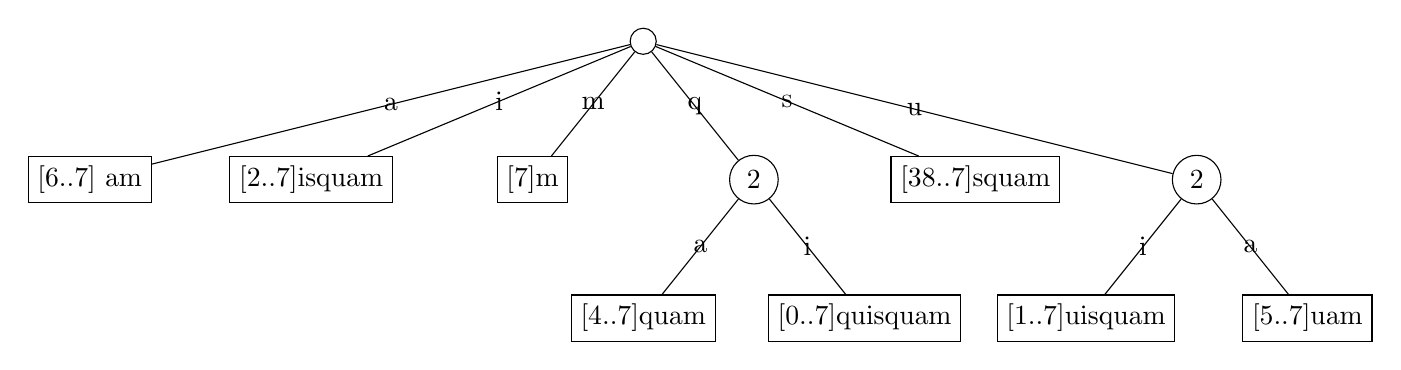
\begin{tikzpicture}[level distance=50pt,
      every node/.style={,circle,draw},
      level 1/.style={sibling distance=80pt},
      level 2/.style={sibling distance=80pt},
      level 3/.style={sibling distance=25pt}]
      \node{}
      child{
        node[rectangle]{[6..7] am}
        edge from parent node[draw=none]{a}
      }
      child{
        node[rectangle]{[2..7]isquam}
        edge from parent node[draw=none]{i}
      }
      child{
        node[rectangle]{[7]m}
        edge from parent node[draw=none]{m}
      }
      child{
        node{2}
        child{
          node[rectangle]{[4..7]quam}
          edge from parent node[draw=none]{a}
        }
        child{
          node[rectangle]{[0..7]quisquam}
          edge from parent node[draw=none]{i}
        }
      edge from parent node[draw=none]{q}
      }
      child{
        node[rectangle]{[38..7]squam}
        edge from parent node[draw=none]{s}
      }
      child{
        node{2}
        child{
          node[rectangle]{[1..7]uisquam}
         edge from parent node[draw=none]{i}
        }
        child{
          node[rectangle]{[5..7]uam}
         edge from parent node[draw=none]{a}
        }
        edge from parent node[draw=none]{u}
      }
      ;
\end{tikzpicture}
\end{center}

%%%%%%%%%%%%%%%%%%%%%%%%%%%%%%%%%%%%%%%%%%%%%%%%%%%%%%%%%%%%%
\subsection{Lempel-Ziv compression [8+1+1+1=11 marks]}
After writing his memoirs, Foghorn Leghorn has decided to compress them
using Lempel-Ziv compression with six bit codes.
The code table is initialized with the codes
$(a,000000)$, $(b,000001)$, $\dots$, $(z,011001)$, $({\vs},011010)$,
$(',011011)$, $(, ,011100)$.
\begin{enumerate}
\part{a}Give the sequence of substrings that will be used during the compression
of the opening sentence ``that's a joke, that's a joke, son, that's a joke''.
If we consider the example of Slide 26 of Module 9, we want you to answer
$$[Y,O,!,{\vs},YO,U,!{\vs},YOU,R,{\vs}Y,O,YO,!].$$

You can assume that the dictionary is big enough to store
all the substrings that we will encounter.

\begin{sideways}
\begin{tabular}{|c|}
  \hline
  T\\
  \hline
  H\\
  \hline
  A\\
  \hline
  T\\
  \hline
  '\\
  \hline
  S\\
  \hline
  \_\\
  \hline
  A\\
  \hline
  \_\\
  \hline
  J\\
  \hline
  O\\
  \hline
  K\\
  \hline
  E\\
  \hline
  ,\\
  \hline
  \_\\
  \hline
  TH\\
  \hline
  AT\\
  \hline
  'S\\
  \hline
  \_A\\
  \hline
   \_J\\
 \hline
 OK\\
 \hline
 E,\\
 \hline
 \_\\
 \hline
 S\\
 \hline
 O\\
 \hline
 N\\
 \hline
 ,\_\\
 \hline
 THA\\
 \hline
 T'\\
 \hline
 S\_\\
 \hline
 A\_\\
 \hline
 JO\\
 \hline
 KE\\
 \hline
\end{tabular}
\end{sideways}


\part{b} What is the size in bits of the classical encoding of the original string considering that we would code every character from $a$ to `,' on 5 bits if we were not using LZW  ?

5 bits * 48 characters = 240

\part{c} What is the size in bits of the compressed string ?

6 bits * 33 characters = 198

\part{d} Given the amount of repetition in the sentence above, comment on the quality of compression of LZW on this instance.

Even though the number of bits per character increases we can see that in numerous places the repetition of character sequences allows us to encode multiple characters under one encoded character. This allows for a compression factor of $\frac{240}{198} = 1.2$.

\end{enumerate}
\end{document}
